%Chapter 3

\chapter{System Design}

\label{Chapter3}
This chapter is about the methodology behind the program and some of the features and requirements.

\section{Method}
The core part of the system will be deciding whether the account it is checking is a bot or not. It will use a form of machine learning to classify the account as either 'bot' or 'not bot'. Initially it would seem as if this was a binary classification issue, however it makes more sense to treat it as a regression problem. This makes it much easier to interpret the results for the user as a probability is easily understood and is a much more honest answer compared to just giving the user a 'yes' or 'no' since we can never be too sure either way.


\section{System Requirements}
In order to achieve the aims of the system, there are a few things the program will need to do.
\begin{enumerate}
	\item Allow users to input a Twitter account.
	\item A connection using the Twitter API must be established in order to retrieve users' data.
	\item The system must be able to determine whether an account is a bot or not.
	\item Display the likelihood that an account is a bot or not.
\end{enumerate}

\section{Algorithm}
The algorithm for my system will consist of a supervised machine learning algorithm called random forest. This works by creating a multitude of decision trees and outputting the mean prediction of these trees. However, depending on how things go during development, it might make more sense to use a deep learning neural network instead for the regression. 

\subsection{Random Forest}
Random forest is a supervised learning algorithm. This means the data must be labelled, otherwise the algorithm won't know what to do with it. It's a useful algorithm, as it can be utilized for both classification and regression problems. In order to understand and implement the random forest algorithm, we first need to know about its building blocks, the decision tree.\\ 
A decision tree is made up of an ensemble of branches and leaves. The branches contain the decisions, whilst the leaves determine the label that the tree believes the data belongs to. These decisions are made based on the features that best help us determine what label the data belongs to. A major downside to decision trees is that they suffer from overfitting when they become too deep with many branches.\\ 
This is where random forest comes in. As the name implies, it combines many decision trees into a forest like object where each trees outcome is thrown together and averaged out to get one answer. However, the clever thing it manages to do is the random feature selection. Each tree takes a limited number of random features from the original total and creates its own decision tree based on that. This helps it give a much more accurate result and mostly remove the overfitting aspect of the algorithm. The other form of randomness comes from the random subset of data selected with replacement for each individual tree, also known as bagging.\\
Once the subsets are decided upon and the trees are split up we must go through the nodes and decide on how to set these rules and which features to base them on. This is done using the gini impurity equation. It's the probability of any given node that a randomly selected sample would be incorrectly labelled if it was labelled by the distribution of samples in that node \cite{DataScience001}.
The gini impurity is worked out using the following equation:
\begingroup
\fontsize{20pt}{10pt}
$$ I_{G}(n) = 1 - \sum_{i=1}^{J}(p_{i}) $$
\endgroup
The gini impurity of a node $n$ is 1 minus the sum over all the classes $J$ of the fraction of examples in each class $p_{i}$ squared \cite{DataScience001}. At nodes beyond the root the gini impurity is additionally weighted by the fraction of points from its parent node. As it is the probability of incorrect labelling, we are looking for values as small as possible here. This is repeated throughout the algorithm recursively, finding the best possible values for the best features to pick until a given depth or if there is only one class' samples remaining. 
\\
\\
%make sure layout is correct here
\clearpage
To further help understand the algorithm it's crucial that we look at the pseudocode as that's much easier to translate into code.
\\
\begin{figure}[h]
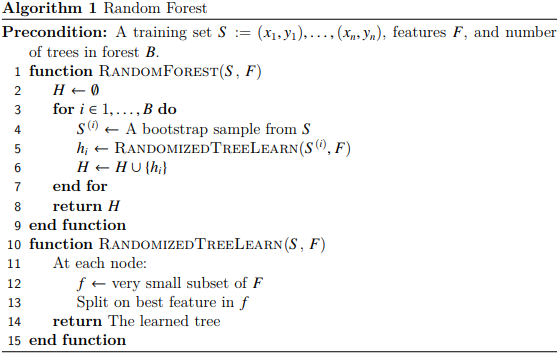
\includegraphics[width=150mm,height=100mm]{figures/pseudocode}
\caption{Random forest pseudocode}
\end{figure}
\\

As previously mentioned, the algorithm works by creating a forest of decision trees. This means that for B number of trees we take a bootstrap or bagging sample of features from the original data and create these decision trees by splitting the nodes on the best features. Once this has been complete all the way down the trees recursively, we return the finished trees and decide based on majority vote which outcome is the most likely. 
\\
\\
\clearpage
To give a visual representation of a decision tree it would look something like the following:
\begin{figure}[h]
	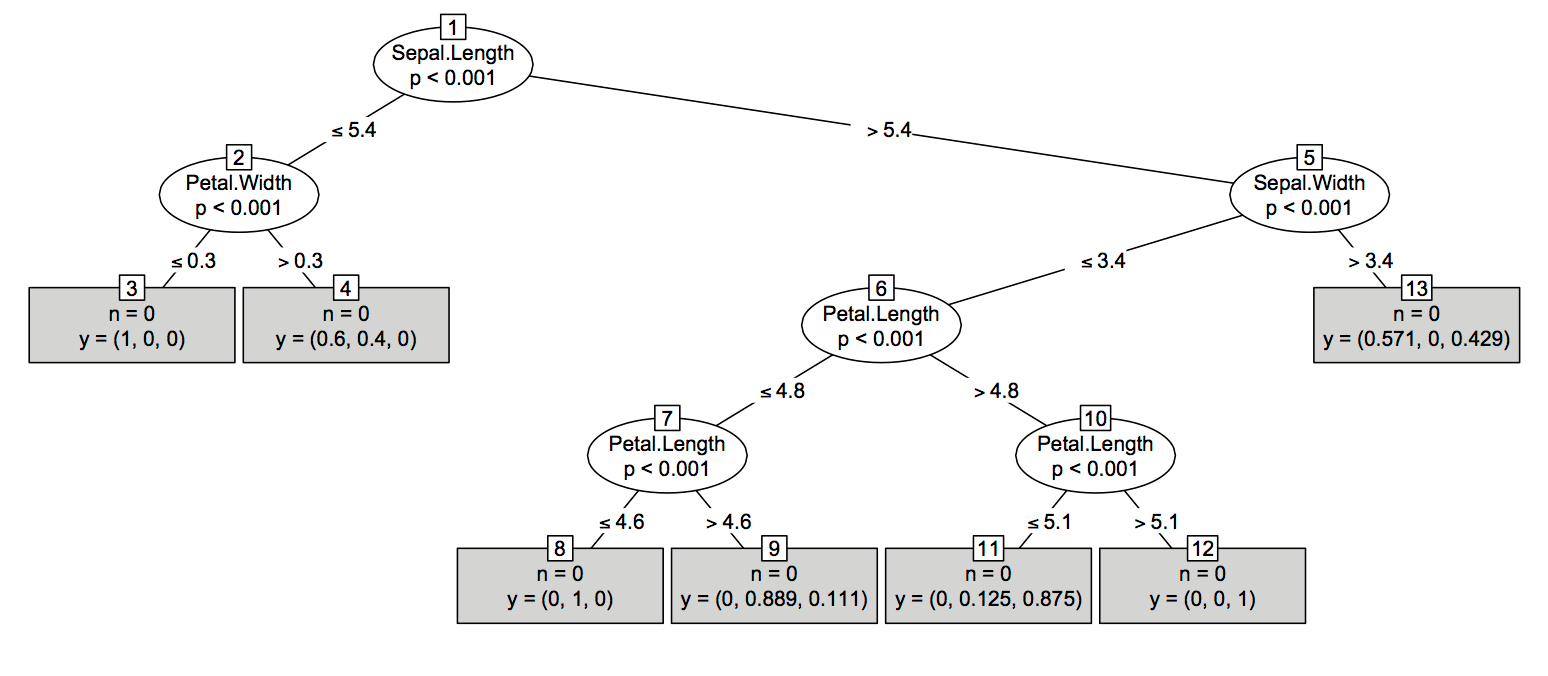
\includegraphics[width=150mm]{figures/tree}
	\caption{An example decision tree using the iris dataset}
\end{figure}
\\
Here you can see that at each node there is a condition being made. This is the 'best' feature that is decided based on the earlier mentioned gini impurity being minimised. Then based on the value of these features for a given datapoint, the algorithm will traverse down a branch of the tree all the way to a root node. This then gives us our prediction for that one decision tree within the forest. 

\subsection{Data}
Regardless of which algorithm I end up finalising with, I will need data for training. This is important since everything will be based on it. This data needs to also be correctly labelled and will most likely need to be pre-processed somewhat before being fed to my algorithm. It will then be used to train the system.

\subsection{Twitter API}
As the user will be able to enter a Twitter account name themselves, the program will need to have Twitter REST API functionality. This is to access the relevant accounts information such as tweets and account details. There is a limited number of requests allowed within a 15 minute window therefore I need to make sure to keep the API requests to a bare minimum. 

